\documentclass[11pt,a4paper]{article}

% ============================================================================
% PACKAGES
% ============================================================================
\usepackage[utf8]{inputenc}
\usepackage[T1]{fontenc}
\usepackage{lmodern}
\usepackage[margin=1in]{geometry}
\usepackage{xcolor}
\usepackage{graphicx}
\usepackage{hyperref}
\usepackage{listings}
\usepackage{tcolorbox}
\usepackage{enumitem}
\usepackage{fontawesome5}
\usepackage{tikz}
\usepackage{fancyhdr}
\usepackage{titlesec}
\usepackage{booktabs}
\usepackage{multicol}
\usepackage{framed}
\usepackage{mdframed}
\usepackage{float}

% ============================================================================
% COLORS
% ============================================================================
\definecolor{primaryblue}{RGB}{37, 99, 235}
\definecolor{secondaryblue}{RGB}{59, 130, 246}
\definecolor{accentgreen}{RGB}{16, 185, 129}
\definecolor{warningorange}{RGB}{245, 158, 11}
\definecolor{dangerred}{RGB}{239, 68, 68}
\definecolor{darkgray}{RGB}{31, 41, 55}
\definecolor{lightgray}{RGB}{243, 244, 246}
\definecolor{codebg}{RGB}{249, 250, 251}
\definecolor{terminalgreen}{RGB}{34, 197, 94}

% ============================================================================
% HYPERREF SETUP
% ============================================================================
\hypersetup{
    colorlinks=true,
    linkcolor=primaryblue,
    urlcolor=secondaryblue,
    pdftitle={BiLSTM-CRF NER Project - Handoff Guide for Hassan},
    pdfauthor={Yasser Hamdan}
}

% ============================================================================
% CODE LISTINGS SETUP
% ============================================================================
\lstset{
    backgroundcolor=\color{codebg},
    basicstyle=\ttfamily\small,
    breaklines=true,
    frame=single,
    rulecolor=\color{lightgray},
    numbers=none,
    showstringspaces=false,
    tabsize=2,
    captionpos=b
}

\lstdefinestyle{terminal}{
    backgroundcolor=\color{darkgray},
    basicstyle=\ttfamily\small\color{white},
    breaklines=true,
    frame=none,
    numbers=none
}

% ============================================================================
% CUSTOM BOXES
% ============================================================================
\newtcolorbox{infobox}{
    colback=primaryblue!5,
    colframe=primaryblue,
    fonttitle=\bfseries,
    title={\faInfoCircle\ Important},
    rounded corners,
    boxrule=1pt
}

\newtcolorbox{warningbox}{
    colback=warningorange!10,
    colframe=warningorange,
    fonttitle=\bfseries,
    title={\faExclamationTriangle\ Warning},
    rounded corners,
    boxrule=1pt
}

\newtcolorbox{successbox}{
    colback=accentgreen!10,
    colframe=accentgreen,
    fonttitle=\bfseries,
    title={\faCheckCircle\ Success},
    rounded corners,
    boxrule=1pt
}

\newtcolorbox{commandbox}{
    colback=darkgray,
    colframe=darkgray,
    fonttitle=\bfseries\color{white},
    coltitle=white,
    title={\faTerminal\ Terminal},
    rounded corners,
    boxrule=0pt
}

\newtcolorbox{taskbox}[1]{
    colback=primaryblue!5,
    colframe=primaryblue,
    fonttitle=\bfseries,
    title={\faClipboardCheck\ Task: #1},
    rounded corners,
    boxrule=1pt
}

% ============================================================================
% HEADER/FOOTER
% ============================================================================
\pagestyle{fancy}
\fancyhf{}
\fancyhead[L]{\textcolor{primaryblue}{\textbf{BiLSTM-CRF NER Project}}}
\fancyhead[R]{\textcolor{gray}{Guide for Hassan}}
\fancyfoot[C]{\thepage}
\renewcommand{\headrulewidth}{2pt}
\renewcommand{\headrule}{\hbox to\headwidth{\color{primaryblue}\leaders\hrule height \headrulewidth\hfill}}

% ============================================================================
% TITLE FORMATTING
% ============================================================================
\titleformat{\section}
    {\Large\bfseries\color{primaryblue}}
    {\thesection}{1em}{}[\color{primaryblue}\titlerule]

\titleformat{\subsection}
    {\large\bfseries\color{darkgray}}
    {\thesubsection}{1em}{}

% ============================================================================
% DOCUMENT
% ============================================================================
\begin{document}

% ============================================================================
% TITLE PAGE
% ============================================================================
\begin{titlepage}
    \centering
    \vspace*{1cm}

    {\Huge\bfseries\color{primaryblue} BiLSTM-CRF NER Project\par}
    \vspace{0.5cm}
    {\LARGE\color{darkgray} Biomedical Named Entity Recognition\par}

    \vspace{1cm}

    
\begin{tikzpicture}
        \draw[fill=primaryblue!10, draw=primaryblue, rounded corners=10pt, line width=2pt]
            (0,0) rectangle (12,2.5);
        \node at (6,1.25) {\Huge\color{primaryblue}\faGithub\ \faArrowRight\ \faPython\ \faArrowRight\ \faRocket};
    \end{tikzpicture}

    \vspace{1.5cm}

    {\Huge\bfseries Complete Setup \& Task Guide\par}
    \vspace{0.5cm}
    {\LARGE For: \textbf{Hassan Najdi}\par}

    \vspace{1.5cm}

    \begin{tcolorbox}[
        colback=accentgreen!10,
        colframe=accentgreen,
        width=0.85\textwidth,
        rounded corners
    ]
        \centering
        \Large\textbf{GitHub Repository:}\\[0.5em]
        \texttt{\large https://github.com/hamdanyasser/NLP-NER-Project}
    \end{tcolorbox}

    \vspace{1.5cm}

    \begin{tcolorbox}[
        colback=lightgray,
        colframe=darkgray,
        width=0.7\textwidth,
        rounded corners
    ]
        \centering
        \textbf{From:} Yasser Hamdan\\[0.3em]
        \textbf{Course:} NLP Final Project\\[0.3em]
        \textbf{Date:} January 2026
    \end{tcolorbox}

    \vfill

    {\large\color{gray} Follow this guide step-by-step to set up, test, and improve the project\par}

\end{titlepage}

% ============================================================================
% TABLE OF CONTENTS
% ============================================================================
\tableofcontents
\newpage

% ============================================================================
% SECTION 1: QUICK START (5 MINUTES)
% ============================================================================
\section{Quick Start - Get Running in 5 Minutes}

\begin{successbox}
Follow these steps exactly in order. Copy-paste the commands.
\end{successbox}

\subsection{Step 1: Clone the Repository}

\begin{commandbox}
\texttt{\textcolor{terminalgreen}{>} git clone https://github.com/hamdanyasser/NLP-NER-Project.git}\\
\texttt{\textcolor{terminalgreen}{>} cd NLP-NER-Project}
\end{commandbox}

\subsection{Step 2: Create Virtual Environment}

\begin{commandbox}
\texttt{\textcolor{terminalgreen}{>} python -m venv venv}
\end{commandbox}

\subsection{Step 3: Activate Virtual Environment}

\textbf{On Windows:}
\begin{commandbox}
\texttt{\textcolor{terminalgreen}{>} venv\textbackslash Scripts\textbackslash activate}
\end{commandbox}

\textbf{On Mac/Linux:}
\begin{commandbox}
\texttt{\textcolor{terminalgreen}{\$} source venv/bin/activate}
\end{commandbox}

You should see \texttt{(venv)} at the start of your prompt.

\subsection{Step 4: Install Dependencies}

\begin{commandbox}
\texttt{\textcolor{terminalgreen}{(venv) >} pip install -r requirements.txt}
\end{commandbox}

\begin{warningbox}
This takes 5-10 minutes. It downloads PyTorch and other packages.
\end{warningbox}

\subsection{Step 5: Verify Everything Works}

\begin{commandbox}
\texttt{\textcolor{terminalgreen}{(venv) >} python demo.py --text "Aspirin causes stomach bleeding"}
\end{commandbox}

\begin{successbox}
If you see entity predictions, you're ready! Move to Section 2.
\end{successbox}

\newpage

% ============================================================================
% SECTION 2: PROJECT OVERVIEW
% ============================================================================
\section{What Is This Project?}

\subsection{Purpose}

This is a \textbf{Named Entity Recognition (NER)} system that finds medical entities in text:

\begin{itemize}[leftmargin=2cm]
    \item[\textcolor{secondaryblue}{\faPills}] \textbf{Chemicals} -- drugs, compounds (Aspirin, Metformin, Penicillin)
    \item[\textcolor{dangerred}{\faHeartbeat}] \textbf{Diseases} -- conditions, symptoms (diabetes, cancer, bleeding)
\end{itemize}

\textbf{Example:}
\begin{lstlisting}
Input:  "Aspirin can cause gastrointestinal bleeding"
Output: [Aspirin] = Chemical
        [gastrointestinal bleeding] = Disease
\end{lstlisting}

\subsection{Architecture}

The model uses \textbf{BiLSTM-CRF} with these components:

\begin{center}
\begin{tabular}{lll}
\toprule
\textbf{Component} & \textbf{What It Does} & \textbf{File} \\
\midrule
Word Embeddings & Converts words to vectors & \texttt{bilstm\_crf.py} \\
Character CNN & Captures word structure & \texttt{layers.py} \\
BiLSTM & Reads context both directions & \texttt{bilstm\_crf.py} \\
Self-Attention & Focuses on important words & \texttt{attention.py} \\
CRF Layer & Ensures valid tag sequences & \texttt{layers.py} \\
\bottomrule
\end{tabular}
\end{center}

\begin{infobox}
Everything is built \textbf{from scratch} in PyTorch -- no external NER libraries. This is important for the course project!
\end{infobox}

\subsection{Current Status}

\begin{center}
\begin{tabular}{lcc}
\toprule
\textbf{Component} & \textbf{Status} & \textbf{Notes} \\
\midrule
Model Implementation & \textcolor{accentgreen}{\faCheckCircle} Done & All layers working \\
Training Pipeline & \textcolor{accentgreen}{\faCheckCircle} Done & With checkpoints \\
Evaluation Metrics & \textcolor{accentgreen}{\faCheckCircle} Done & P/R/F1 \\
Unit Tests & \textcolor{accentgreen}{\faCheckCircle} Done & 37+ tests \\
Demo (CLI + Web) & \textcolor{accentgreen}{\faCheckCircle} Done & Both working \\
\midrule
Train on Full Dataset & \textcolor{warningorange}{\faExclamationCircle} Needed & Currently sample data \\
Improve F1 Score & \textcolor{warningorange}{\faExclamationCircle} Needed & Target: 85\%+ \\
Final Report & \textcolor{warningorange}{\faExclamationCircle} Needed & Write-up \\
\bottomrule
\end{tabular}
\end{center}

\newpage

% ============================================================================
% SECTION 3: YOUR TASKS
% ============================================================================
\section{Your Tasks - What To Do}

\begin{infobox}
Use \textbf{Claude Code} (AI assistant) to help you with these tasks. It can write code, fix bugs, and explain things. See Section 5 for how to use it.
\end{infobox}

\subsection{Task 1: Run Tests (Verify Everything Works)}

\begin{taskbox}{Run Unit Tests}
\begin{commandbox}
\texttt{\textcolor{terminalgreen}{(venv) >} python -m pytest tests/ -v}
\end{commandbox}

\textbf{Expected:} All tests pass (37 passed, maybe 1 skipped)

\textbf{If tests fail:} Ask Claude Code to fix them.
\end{taskbox}

\subsection{Task 2: Train the Model}

\begin{taskbox}{Train on Current Data}
\begin{commandbox}
\texttt{\textcolor{terminalgreen}{(venv) >} python -m src.training.train --config config/config.yaml}
\end{commandbox}

\textbf{Expected:} Training runs for 10 epochs, saves model to \texttt{artifacts/}

\textbf{Watch for:} Loss should decrease each epoch.
\end{taskbox}

\subsection{Task 3: Evaluate the Model}

\begin{taskbox}{Check Performance}
\begin{commandbox}
\texttt{\textcolor{terminalgreen}{(venv) >} python -m src.training.eval --config config/config.yaml}
\end{commandbox}

\textbf{Expected:} Shows Precision, Recall, F1 scores

\textbf{Current F1:} ~13\% (low because of small sample data)
\end{taskbox}

\subsection{Task 4: Improve Performance (MAIN TASK)}

The current model is trained on only ~280 sample sentences. To get good results:

\begin{taskbox}{Download Real BC5CDR Dataset}
Ask Claude Code:
\begin{mdframed}[backgroundcolor=lightgray, linewidth=0pt]
\texttt{"Download the real BC5CDR dataset from the official source, parse it correctly, and retrain the model. Target F1 score should be 85\%+"}
\end{mdframed}
\end{taskbox}

\begin{taskbox}{Add GloVe Embeddings}
Ask Claude Code:
\begin{mdframed}[backgroundcolor=lightgray, linewidth=0pt]
\texttt{"Download GloVe 100d embeddings and enable them in the config. This should improve performance."}
\end{mdframed}
\end{taskbox}

\begin{taskbox}{Run Ablation Study}
Ask Claude Code:
\begin{mdframed}[backgroundcolor=lightgray, linewidth=0pt]
\texttt{"Run the ablation study to compare different model configurations and generate a results table."}
\end{mdframed}
\end{taskbox}

\subsection{Task 5: Test the Demo}

\begin{taskbox}{Interactive Demo}
\begin{commandbox}
\texttt{\textcolor{terminalgreen}{(venv) >} python demo.py}
\end{commandbox}

Type sentences like:
\begin{itemize}
    \item "Metformin is used to treat diabetes"
    \item "Ibuprofen may cause kidney damage"
    \item "Penicillin allergies can cause anaphylaxis"
\end{itemize}
\end{taskbox}

\begin{taskbox}{Web Demo (Optional)}
\begin{commandbox}
\texttt{\textcolor{terminalgreen}{(venv) >} pip install gradio}\\
\texttt{\textcolor{terminalgreen}{(venv) >} python app.py}
\end{commandbox}

Open \url{http://localhost:7860} in browser.
\end{taskbox}

\newpage

% ============================================================================
% SECTION 4: GIT WORKFLOW
% ============================================================================
\section{Git Workflow - How To Collaborate}

\subsection{Before You Start Working}

Always pull the latest changes:

\begin{commandbox}
\texttt{\textcolor{terminalgreen}{(venv) >} git pull origin main}
\end{commandbox}

\subsection{After You Make Changes}

\begin{commandbox}
\texttt{\textcolor{terminalgreen}{(venv) >} git add .}\\
\texttt{\textcolor{terminalgreen}{(venv) >} git commit -m "Description of what you changed"}\\
\texttt{\textcolor{terminalgreen}{(venv) >} git push origin main}
\end{commandbox}

\subsection{Example Workflow}

\begin{enumerate}
    \item \texttt{git pull origin main} -- Get latest changes
    \item Make your changes (or ask Claude Code to help)
    \item Test that it works: \texttt{python -m pytest tests/ -v}
    \item \texttt{git add .} -- Stage changes
    \item \texttt{git commit -m "Added GloVe embeddings"} -- Commit
    \item \texttt{git push origin main} -- Push to GitHub
\end{enumerate}

\begin{warningbox}
Always \texttt{git pull} before starting work to avoid conflicts!
\end{warningbox}

\subsection{If You Get Merge Conflicts}

Ask Claude Code:
\begin{mdframed}[backgroundcolor=lightgray, linewidth=0pt]
\texttt{"I have a git merge conflict. Can you help me resolve it?"}
\end{mdframed}

\newpage

% ============================================================================
% SECTION 5: USING CLAUDE CODE
% ============================================================================
\section{Using Claude Code (AI Assistant)}

\subsection{What Is Claude Code?}

Claude Code is an AI that can:
\begin{itemize}
    \item Read and understand your entire codebase
    \item Write and edit code
    \item Run terminal commands
    \item Debug and fix issues
    \item Explain how things work
\end{itemize}

\subsection{Installing Claude Code}

\textbf{Step 1:} Install Node.js from \url{https://nodejs.org/} (LTS version)

\textbf{Step 2:} Install Claude Code:
\begin{commandbox}
\texttt{\textcolor{terminalgreen}{>} npm install -g @anthropic-ai/claude-code}
\end{commandbox}

\textbf{Step 3:} Run it in your project folder:
\begin{commandbox}
\texttt{\textcolor{terminalgreen}{>} cd path/to/NLP-NER-Project}\\
\texttt{\textcolor{terminalgreen}{>} claude}
\end{commandbox}

\textbf{Step 4:} Login with your Anthropic account when prompted.

\subsection{Useful Prompts for This Project}

Copy-paste these prompts into Claude Code:

\begin{mdframed}[backgroundcolor=primaryblue!5, linewidth=1pt, linecolor=primaryblue]
\textbf{Understand the project:}\\
\texttt{"Explain the architecture of this BiLSTM-CRF NER project"}
\end{mdframed}

\begin{mdframed}[backgroundcolor=primaryblue!5, linewidth=1pt, linecolor=primaryblue]
\textbf{Run tests:}\\
\texttt{"Run all the tests and fix any that fail"}
\end{mdframed}

\begin{mdframed}[backgroundcolor=primaryblue!5, linewidth=1pt, linecolor=primaryblue]
\textbf{Train model:}\\
\texttt{"Train the model and show me the results"}
\end{mdframed}

\begin{mdframed}[backgroundcolor=primaryblue!5, linewidth=1pt, linecolor=primaryblue]
\textbf{Improve performance:}\\
\texttt{"The F1 score is too low. Analyze the issues and suggest improvements"}
\end{mdframed}

\begin{mdframed}[backgroundcolor=primaryblue!5, linewidth=1pt, linecolor=primaryblue]
\textbf{Fix errors:}\\
\texttt{"I'm getting this error: [paste error]. Fix it."}
\end{mdframed}

\begin{mdframed}[backgroundcolor=primaryblue!5, linewidth=1pt, linecolor=primaryblue]
\textbf{Download real dataset:}\\
\texttt{"Download the BC5CDR dataset and retrain with it"}
\end{mdframed}

\newpage

% ============================================================================
% SECTION 6: COMMAND REFERENCE
% ============================================================================
\section{Command Reference}

\begin{center}
\begin{tabular}{p{5.5cm}p{8.5cm}}
\toprule
\textbf{What You Want To Do} & \textbf{Command} \\
\midrule
\multicolumn{2}{l}{\textbf{Setup}} \\
\midrule
Clone repository & \texttt{git clone <URL>} \\
Create virtual env & \texttt{python -m venv venv} \\
Activate (Windows) & \texttt{venv\textbackslash Scripts\textbackslash activate} \\
Activate (Mac/Linux) & \texttt{source venv/bin/activate} \\
Install dependencies & \texttt{pip install -r requirements.txt} \\
\midrule
\multicolumn{2}{l}{\textbf{Testing}} \\
\midrule
Run all tests & \texttt{python -m pytest tests/ -v} \\
Run specific test file & \texttt{python -m pytest tests/test\_model.py -v} \\
\midrule
\multicolumn{2}{l}{\textbf{Training \& Evaluation}} \\
\midrule
Train model & \texttt{python -m src.training.train} \\
Evaluate model & \texttt{python -m src.training.eval} \\
Quick test (3 epochs) & \texttt{python -m src.training.train --config config/config\_test.yaml} \\
\midrule
\multicolumn{2}{l}{\textbf{Demo}} \\
\midrule
Interactive CLI & \texttt{python demo.py} \\
Single text & \texttt{python demo.py --text "your text"} \\
Web demo & \texttt{python app.py} \\
\midrule
\multicolumn{2}{l}{\textbf{Git}} \\
\midrule
Pull latest & \texttt{git pull origin main} \\
Stage changes & \texttt{git add .} \\
Commit & \texttt{git commit -m "message"} \\
Push & \texttt{git push origin main} \\
Check status & \texttt{git status} \\
\bottomrule
\end{tabular}
\end{center}

\newpage

% ============================================================================
% SECTION 7: PROJECT STRUCTURE
% ============================================================================
\section{Project Structure}

\begin{lstlisting}[basicstyle=\ttfamily\footnotesize]
NLP-NER-Project/
|
|-- config/
|   +-- config.yaml           # Main settings (epochs, learning rate, etc.)
|
|-- src/
|   |-- data/
|   |   |-- preprocess.py     # Data preparation
|   |   +-- dataset.py        # PyTorch Dataset
|   |
|   |-- models/
|   |   |-- bilstm_crf.py     # Main model (THIS IS THE CORE)
|   |   |-- layers.py         # CRF layer (from scratch!)
|   |   +-- attention.py      # Self-attention
|   |
|   |-- training/
|   |   |-- train.py          # Training loop
|   |   +-- eval.py           # Evaluation
|   |
|   +-- utils/
|       |-- metrics.py        # F1, Precision, Recall
|       +-- vocab.py          # Word/label vocabularies
|
|-- tests/                    # Unit tests
|-- artifacts/                # Saved models
|-- data/processed/           # Training data
|-- demo.py                   # CLI demo
|-- app.py                    # Web demo
+-- requirements.txt          # Dependencies
\end{lstlisting}

\newpage

% ============================================================================
% SECTION 8: TROUBLESHOOTING
% ============================================================================
\section{Troubleshooting}

\begin{center}
\begin{tabular}{p{4.5cm}p{9.5cm}}
\toprule
\textbf{Problem} & \textbf{Solution} \\
\midrule
\texttt{ModuleNotFoundError} & Activate venv: \texttt{venv\textbackslash Scripts\textbackslash activate} \\
\midrule
\texttt{No module named torch} & Run: \texttt{pip install -r requirements.txt} \\
\midrule
Model not found & Train first: \texttt{python -m src.training.train} \\
\midrule
CUDA out of memory & Edit \texttt{config/config.yaml}, reduce \texttt{batch\_size} to 8 \\
\midrule
Tests failing & Ask Claude Code: "Fix the failing tests" \\
\midrule
Git conflict & Ask Claude Code: "Help me resolve git conflicts" \\
\midrule
Low F1 score & Need more training data - see Task 4 in Section 3 \\
\bottomrule
\end{tabular}
\end{center}

\vspace{1cm}

\begin{infobox}
For any problem, just describe it to Claude Code:\\[0.5em]
\texttt{"I'm getting this error: [paste error]. What's wrong and how do I fix it?"}
\end{infobox}

\newpage

% ============================================================================
% SECTION 9: CHECKLIST
% ============================================================================
\section{Complete Checklist}

\begin{center}
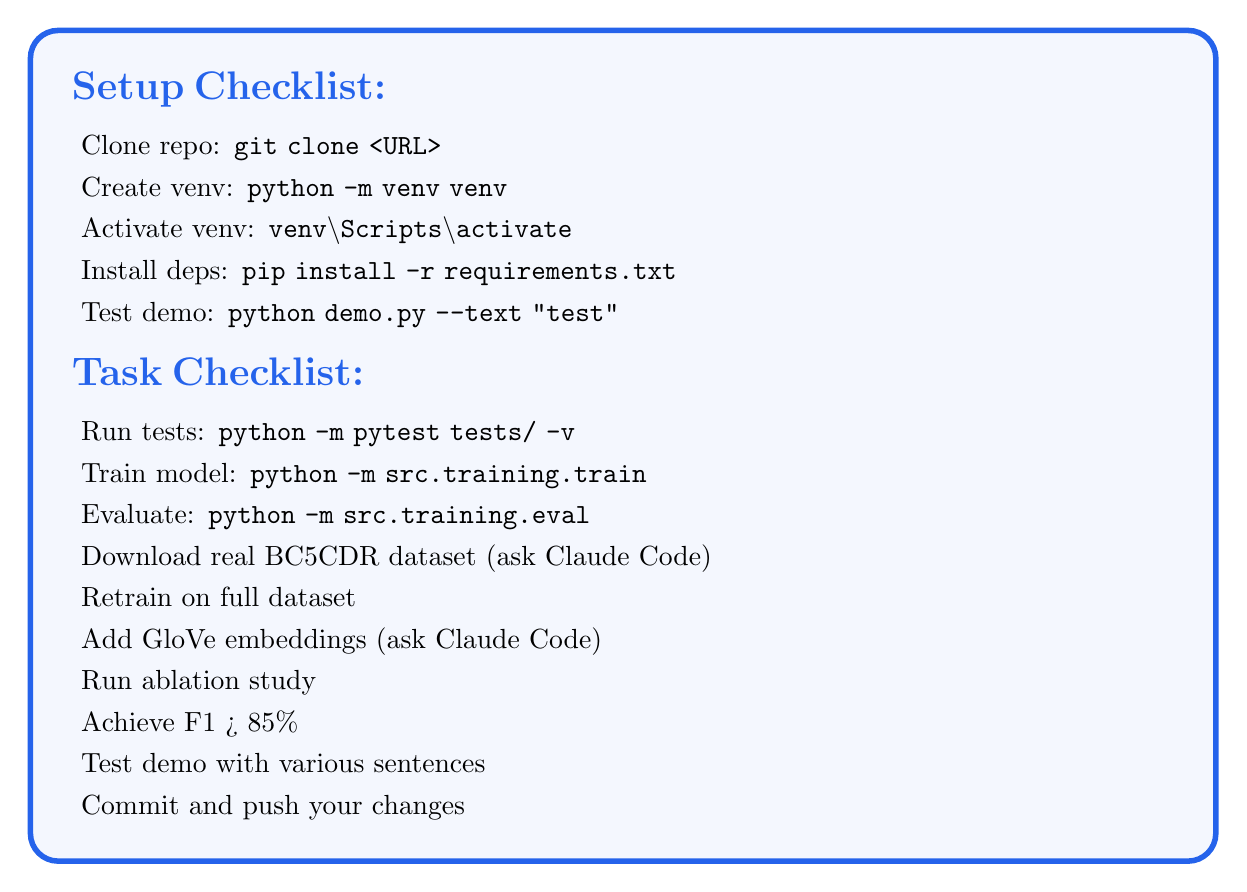
\begin{tikzpicture}
\node[draw=primaryblue, fill=primaryblue!5, rounded corners=10pt, line width=2pt,
      text width=14cm, align=left, inner sep=15pt] {
    \textbf{\Large\color{primaryblue} Setup Checklist:}\\[0.8em]

    $\square$ Clone repo: \texttt{git clone <URL>}\\[0.3em]
    $\square$ Create venv: \texttt{python -m venv venv}\\[0.3em]
    $\square$ Activate venv: \texttt{venv\textbackslash Scripts\textbackslash activate}\\[0.3em]
    $\square$ Install deps: \texttt{pip install -r requirements.txt}\\[0.3em]
    $\square$ Test demo: \texttt{python demo.py --text "test"}\\[1em]

    \textbf{\Large\color{primaryblue} Task Checklist:}\\[0.8em]

    $\square$ Run tests: \texttt{python -m pytest tests/ -v}\\[0.3em]
    $\square$ Train model: \texttt{python -m src.training.train}\\[0.3em]
    $\square$ Evaluate: \texttt{python -m src.training.eval}\\[0.3em]
    $\square$ Download real BC5CDR dataset (ask Claude Code)\\[0.3em]
    $\square$ Retrain on full dataset\\[0.3em]
    $\square$ Add GloVe embeddings (ask Claude Code)\\[0.3em]
    $\square$ Run ablation study\\[0.3em]
    $\square$ Achieve F1 > 85\%\\[0.3em]
    $\square$ Test demo with various sentences\\[0.3em]
    $\square$ Commit and push your changes\\[0.3em]
};
\end{tikzpicture}
\end{center}

\vspace{1.5cm}

\begin{center}
\begin{tcolorbox}[
    colback=accentgreen!10,
    colframe=accentgreen,
    width=0.9\textwidth,
    rounded corners
]
    \centering
    \Large\textbf{Good luck, Hassan! \faRocket}\\[0.5em]
    \normalsize Use Claude Code for help -- it knows the entire project.\\[0.5em]
    Contact Yasser if you have questions.\\[1em]
    \textbf{-- Yasser Hamdan}
\end{tcolorbox}
\end{center}

\end{document}
